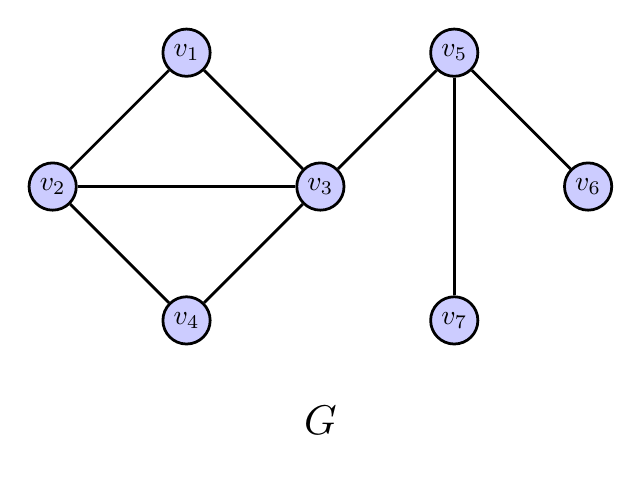
\begin{tikzpicture}[
  scale=0.85, 
  auto=left,
  every node/.style={circle, fill=blue!20, draw=black, line width=1pt, inner sep=2pt, minimum size=6mm}
]

  % Vértices según la disposición del dibujo
  \node (v1) at (2,4) {$v_1$};
  \node (v2) at (0,2) {$v_2$};
  \node (v3) at (4,2) {$v_3$};
  \node (v4) at (2,0) {$v_4$};
  \node (v5) at (6,4) {$v_5$};
  \node (v6) at (8,2) {$v_6$};
  \node (v7) at (6,0) {$v_7$};

  % Aristas de la sección izquierda (entre v1, v2, v3, v4)
  \draw[line width=1pt] (v1) -- (v2);
  \draw[line width=1pt] (v1) -- (v3);
  \draw[line width=1pt] (v2) -- (v3);
  \draw[line width=1pt] (v2) -- (v4);
  \draw[line width=1pt] (v4) -- (v3);

  % Conexión puente (v3 -- v5)
  \draw[line width=1pt] (v3) -- (v5);

  % Aristas de la estrella en v5 (v5 -- v6, v5 -- v7)
  \draw[line width=1pt] (v5) -- (v6);
  \draw[line width=1pt] (v5) -- (v7);

   
  \node[draw=none, fill=none, scale=1.5] at (4,-1.5) {$G$};
\end{tikzpicture}
